Normalerweise wird Java in einem zweistufigen Prozess ausgeführt. Zunächst wird eine plattformabhängige JVM geladen. Innerhalb dieser JVM wird der Java-Compiler (javac) aufgerufen. Dieser compiliert Java-Quelltext zu Java-Bytecode. Der Java-Bytecode kann dann von der JVM ausgeführt werden. Dieser Ablauf ist in der \ref{Abbildung 4.4} unter a) dargestellt.

Um Java in einem Browser auszuführen ergeben sich konzeptionell mindestens drei verschiedene Möglichkeiten, die in \ref{Abbildung 4.4} mit den Buchstaben b-d gekennzeichnet sind.

\begin{figure}[H]
    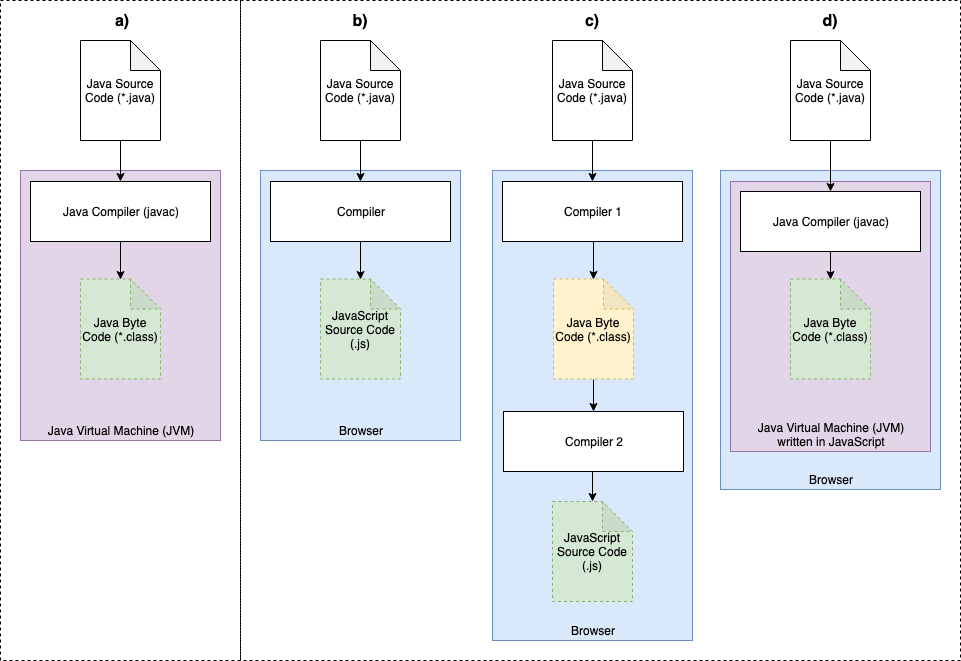
\includegraphics[width=14cm]{chapter/entwurf/Java_JavaScript_Execution.png}
    \centering
    \caption{Blubb}
    \label{Abbildung 4.4}
\end{figure}

\begin{itemize}
    \item \textbf{b):} Java-Quelltext wird mit einem Compiler direkt in JavaScript umgewandelt: Diese Variante ist konzeptionell sehr einfach. Zwar gibt es einige Programme, welche Java-Quelltext in JavaScript übersetzen können (zum Beispiel JSweet oder GWT), jedoch sind alle diese Programme entweder in Java selbst oder in anderen Programmiersprachen verfasst. Einen solchen Compiler, der selbst in JavaScript geschrieben wurde, gibt es bisher nicht. Es wäre möglich eines dieser Programme auf einem separaten Server zu verwenden. Dies würde aber eine weitere Abhängigkeit von einem Server bedeuten, und damit der formulierten Kern-Anforderung widersprechen.
    \item \textbf{c):} Java-Quelltext wird mithilfe eines ersten Compilers in Java-Bytecode übersetzt. Anschließend wird der Java-Bytecode mit einem zweiten Compiler in JavaScript übersetzt. Auch hier ergibt sich das gleiche Problem wie in b). Zwar gibt es Programme, die den jeweiligen Teilschritt übernehmen könnten, jedoch ist keins davon in JavaScript verfasst, so dass es keine Lösung dafür im Browser gibt.
    \item \textbf{d):} Es wird eine JVM verwendet, die in JavaScript implementiert wurde. Mithilfe dieser JVM kann der javac-Compiler geladen werden, um Java-Quelltext in Java-Bytecode zu übersetzen und anschließend auszuprobieren. Mit dem Software-Projekt Doppio fand sich eine überzeugende Implementierung, die relativ einfach eingesetzt werden konnte.Der konzeptionelle Nachteil dieser Lösung liegt in der benötigten Datenmenge: Um eine JVM im Browser auszuführen wird die Java Runtime Environment benötigt, deren Größe bei etwa 60 Megabyte liegt.
\end{itemize}